  \solution{
Implication graph:\medskip

%TCIMACRO{%
%\TeXButton{Decision tree}{\begin{tikzpicture}[node distance=2.5cm,auto]
%\node (D) {D=0@2};
%\node (B) [above right of=D] {B=1@2};
%\node (C) [below right of=D] {C=0@2};
%\node (A) [right of=B] {A=0@1};
%\node (K) [right of=C] {$\mathcal K$};
%\path[->] (D) edge node {$C_2$} (B);
%\path[->] (D) edge node {$C_3$} (C);
%\path[->] (B) edge node {$C_1$} (K);
%\path[->] (C) edge node {$C_1$} (K);
%\path[->] (A) edge node {$C_1$} (K);
%\end{tikzpicture}}}%
%BeginExpansion
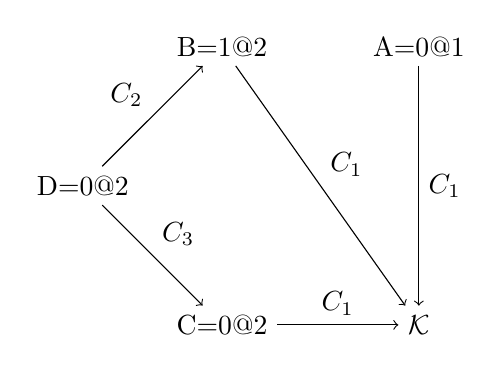
\begin{tikzpicture}[node distance=2.5cm,auto]
\node (D) {D=0@2};
\node (B) [above right of=D] {B=1@2};
\node (C) [below right of=D] {C=0@2};
\node (A) [right of=B] {A=0@1};
\node (K) [right of=C] {$\mathcal K$};
\path[->] (D) edge node {$C_2$} (B);
\path[->] (D) edge node {$C_3$} (C);
\path[->] (B) edge node {$C_1$} (K);
\path[->] (C) edge node {$C_1$} (K);
\path[->] (A) edge node {$C_1$} (K);
\end{tikzpicture}%
%EndExpansion
\newline
\bigskip

  }